\documentclass[aps,onecolumn,preprintnumbers,amsmath,amssymb,nofootinbib,superscriptaddress,notitlepage]{revtex4-1}

\usepackage{graphicx} 
\usepackage{dashrule}
\usepackage{dcolumn} 
\usepackage{mathtools}
\usepackage{amssymb} 
\usepackage{bbold}
\usepackage{amsmath} 
\usepackage{amsfonts} 
\usepackage{wasysym}
\usepackage{slashed} 
\usepackage[dvipsnames]{xcolor} 
\usepackage{soul}
\usepackage{rotating}
\usepackage{paracol}
\usepackage{nicefrac}
\usepackage{MnSymbol}
\usepackage{caption}

\newcommand{\reales}{{\rm R}\hspace{-1ex}\rule{0.1mm}{1.5ex}\hspace{1ex}}
\def\tstrut{\vrule height2.5ex depth0pt width0pt} % used in tables
\def\jtstrut{\vrule height5ex depth0pt width0pt} % used in tables

\newcommand{\figref}[1]{fig.~(\ref{#1})}
\newcommand{\tabref}[1]{table~(\ref{#1})}
\newcommand{\eref}[1]{eq.~(\ref{#1})}
\newcommand{\eg}{\textit{e.g.}~}
\newcommand{\ie}{\textit{i.e.}~}
\newcommand{\viz}{\textit{viz.}~}
\newcommand{\cf}{\textit{cf.}~}
\newcommand{\eftnopi}{\mbox{EFT($\slashed{\pi}$) }} 
\newcommand{\ve}[1]{\ensuremath{\boldsymbol{#1}}}
\newcommand{\rcm}{\ensuremath{\ve{R}_\text{\scriptsize{c.m.}}}}
\newcommand*{\mprime}{^{\prime}\mkern-1.2mu}
\newcommand*{\mdprime}{^{\prime\prime}\mkern-1.2mu}
\newcommand*{\mtprime}{^{\prime\prime\prime}\mkern-1.2mu}
\newcommand{\ddrei}[1]{\delta_{\tiny \lambda}^{(3)}\!\big(#1\big)}
\newcommand{\cc}{\ensuremath C(\lambda)}
\newcommand{\dd}{\ensuremath D(\lambda)}
\newcommand{\hbstwom}{\ensuremath \frac{\hbar^2}{2\mu}}
\newcommand{\twomhbs}{\ensuremath \frac{2\mu}{\hbar^2}}
\newcommand{\coup}[3]{\left[\,#1\,\otimes\,#2\,\right]^{#3}}
\newcommand{\threej}[6]{ \begin{pmatrix}
   #1 & #2 & #3 \\
   #4 & #5 & #6 
  \end{pmatrix}}

\newcommand{\bra}[1] {\left\langle~#1~\right|}
\newcommand{\ket}[1] {\left|~#1~\right\rangle}
\newcommand{\bet}[1] {\left|#1\right|}
\newcommand{\overlap}[2] {\left\langle\,#1\,\left|\,#2\,\right.\right\rangle}
\newcommand{\me}[3] {\left\langle\,#1\,\left.\left|\,#2\,\right|\right.\,#3\,\right\rangle}
\newcommand{\mer}[3] {\left\langle\,#1\,\left|\left.\,#2\,\right|\,#3\,\right.\right\rangle_{\ve{R}}}
\newcommand{\redme}[3] {\left\langle\,#1\,\middle|\right|\,#2\,\left|\middle|\,#3\,\right\rangle}

\definecolor{green}{HTML}{2E8B57}
\interfootnotelinepenalty=10000 %% Completely prevent breaking of footnote

\begin{document}

\section{Appendix: Resonating group method and interactions}


%We treat $A$ as the triton, $B$ as the neutron, and expand the cluster-internal function in a Gaussian basis
%
%\begin{equation}\label{eq.app.trit}
%\phi_3=\sum_n^{N_f}\,c_n\cdot e^{-\alpha_n\sum_{i=1}^{3}\left(\ve{r}_i-\ve{R}_3\right)^2}
%\qquad
%\begin{array}{ll}
%     N_f      & \text{\small : basis dimension}  \\
%     \ve{r}_i & \text{\small : single-particle coordinates}  \\
%     \ve{R}_3 & \text{\small : center of mass of the triton fragment}
%\end{array} 
%\quad,
%\end{equation}
%
%to allow for an analytical reduction of the equation of motion from its full four-body to an
%effective two-body version which assumes that the triton-internal motion is unaffected by the
%scattered neutron.
%
% As we treat the triton as inert, we consider

The non-relativistic dynamics of the four particles is given by the solutions to

\begin{equation}\label{eq.rgm.eqom}
\left(-\frac{\hbar^2}{2\mu}\ve{\Delta}_R-E+\mathcal{V}\right)\ket{\Psi}
~
\Leftrightarrow
~
\me{\delta\Psi}{\hat{H}-E}{\Psi}
=
0
\qquad.
\end{equation}

The second, viz. the projection/variational equation is equivalent to the Schr\"odinger equation if
$\delta\Psi$ denotes an arbitrary variation of the state.
The resonating-group methods expresses the total wave function of this state in the form

\begin{eqnarray}\label{eq.app.rgmwfkt}
\Psi
&=&
\mathcal{A}\Big\lbrace
\sum_i\phi(A_i)\,\phi(B_i)\,\chi_i(\ve{R}_i)
\nonumber\\
&&
+\sum_j\phi(A_j)\,\phi(B_j)\,\phi(C_j)\,\chi_j(\ve{R}_{j1},\ve{R}_{j2})
+\sum_k\phi(A_k)\,\phi(B_k)\,\phi(C_k)\,\phi(D_k)\,\chi_j(\ve{R}_{k1},\ve{R}_{k2},\ve{R}_{k3})
\nonumber\\
&&
+\ldots+\sum_mc_m\eta_m
\Big\rbrace~
\zeta(\rcm)
\qquad,
\end{eqnarray}

where each term corresponds to a particular fragmentation of the particles into two, three, four, $\ldots$ cluster.
The internal motion of such a cluster of $A$ particles is expanded with a complete set of functions $\phi(A_i)$, and the
relative motion between the clusters is encoded in the $\chi_i$'s. The last term is included to improve the expansion if the
fragment-internal basis is not complete and/or if the cluster expansion is truncated such that a more complicated shape
of the state for small separations between the clusters cannot be accounted for.

For the elastic scattering of a neutron off a three-nucleon targets whose ground state is 
$\Delta\epsilon_\text{nuclear}\approx6.2~$MeV and
$\Delta\epsilon_\text{unitary}\approx8.4~$MeV, respectively, below the lowest dissociation thresholds,
and the relative energies between the fragments $E_r\ll\Delta\epsilon$,
we chose to express the wave function of the system with a two-cluster, single-channel ansatz
without specific distortion (\cf\eref{eq.app.rgmwfkt}, first term):

\begin{equation}\label{eq.app.rgmwfkt2}
\Psi
=
\mathcal{A}_{31}\left[\phi(3)\phi(1)\,\chi(\ve{R})\,\zeta(\rcm)\right]
=
\int\mathcal{A}_{31}\left[\phi(3)\phi(1)\,\delta\big(\ve{R}-\ve{R}\mprime\big)\,\zeta(\rcm)\right]\,\chi(\ve{R}\mprime)\,d\ve{R}\mprime
\qquad.
\end{equation}

The parameter representation employed with the second equality in \eref{eq.app.rgmwfkt2}
will yield a defining equation for the relative motion independent of the antisymmetrizer $\mathcal{A}$.
Assuming an inert triton core ammounts to a variation of the relative wave function, only:

\begin{equation}\label{eq.app.rgmwfkt}
\delta\Psi
=
\int\,\delta\chi(\ve{R}\mprime)\,\mathcal{A}_{AB}\left[\phi_A\phi_B\,\delta\big(\ve{R}-\ve{R}\mprime\big)\,\zeta(\rcm)\right]\,d\ve{R}\mprime
\equiv
\sumint \delta a_n\Phi_n
\qquad.
\end{equation}

The latter notation allows for the following concise form of the projection equation

\begin{equation}\label{eq.app.rgmwfkt}
\me{\sumint \delta a_m\Phi_m}{\hat{H}-E}{ \sumint a_n\Phi_n}=0
~\to~\mer{\phi(3)}{\hat{H}-E}{\mathcal{A}_{31}\left[\chi(\ve{R}\mprime)\,\phi(3)\right]}=0
\qquad
\end{equation}

where the {\it ket} subscript average indicates that the average over the relative radius was already taken,
and the remaining integrals are over the fragment-internal coordinates. If the cluster-internal states are properly
anti-symmetrized, it remains to consider the inter-fragment anti-symmetrization via
 $\mathcal{A}_{31}=\mathbb{1}-\hat{P}_{14}$.
We chose nucleons 1 and 4 to be the neutrons with identical spin orientation, and hence need to permutate only
those particles. All other permutations $\hat{P}_{ij}$ will yield zero matrix elements because of the orthogonality of
the internal states.

Being more explicit, the motion of the two fragments relative to each other is approximated by
\begin{equation}\label{eq.rgm.eqom}
\int\left\lbrace~\phi(3)\left(-\frac{\hbar^2}{2\mu}\ve{\Delta}_R-E+B(3)+\mathcal{V}_{31}\right)
\mathcal{A}_{31}\left[\phi(3)\,\chi(\ve{R})\right]\right\rbrace d\ve{r}_{1,2,3}=0
\qquad.
\end{equation}

This expression is further evaluated by:
(i)~employing the parameter representation, $\chi(\ve{R})=\int\delta(\ve{R}-\ve{R}\mprime)\chi(\ve{R}\mprime)d\ve{R}\mprime$;
(ii)~expanding the triton ground state in Gaussians,
$\phi(3)=\sum_n^{N_f}\,c_n\cdot e^{-\alpha_n\sum_{i=1}^3\left(\ve{r}_i-\ve{R}_3\right)^2}$ with norm
$\mathbb{N}_3=\sum_{i,j=1}^{N_f}c_ic_j\left(\frac{\pi}{\alpha_i+\alpha_j}\right)^{\nicefrac{3}{2}}$;
(iii)~substituting the leading-order \eftnopi~potential as inter-cluster interaction,

\begin{eqnarray}\label{eq.app.pot}
\mathcal{V}_{31}
&=&
\cc\,\sum_{i\in A\atop j\in B}\,\ddrei{\ve{r}_i-\ve{r}_j}+
\dd\,\sum_{i,j,k\atop i\in A\Rightarrow j\vee k\in B}\ddrei{\ve{r}_i-\ve{r}_j}\,\ddrei{\ve{r}_i-\ve{r}_k}
\nonumber\\
&=&
\cc\cdot\left(\ddrei{\ve{r}_2-\ve{r}_4}+\ddrei{\ve{r}_3-\ve{r}_4}\right)
+\dd\cdot\left(\ddrei{\ve{r}_2-\ve{r}_3}\,\ddrei{\ve{r}_2-\ve{r}_4}\right)
\qquad;
\end{eqnarray}

(iv)~acting with $\mathcal{A}_{31}$ on $\phi_3$ and $\delta(\ve{R}-\ve{R}\mprime)$;
and finally, (v)~doing the Gaussian integrals for the triton-internal single-particle coordinates $\ve{r}_{1,2,3}$.
Thereby, one obtains the form

\begin{equation}\label{eq.app.rgmform}
(\hat{T}-E)~\chi(\ve{R})+\mathcal{V}^{(1)}(\ve{R})~\chi(\ve{R})+
\int d^{(3)}\ve{R}\mprime~\mathcal{V}^{(2)}(\ve{R},\ve{R}\mprime,E)~\chi(\ve{R}\mprime)=0
\qquad.
\end{equation}

More conveniently, we do express this equation as

\begin{gather}\label{eq.app.rgm.sglnonloc}
\mathbb{N}_3\cdot\left(-\ve{\Delta}_R-\ve{p}^2\right)\,\chi(\ve{R})+
\sum_{i,j=1}^{N_f}c_ic_j\left[
\sum_{n=1}^{2}\eta^{(ij)}_n~e^{-w^{(ij)}_n\ve{R}^2}\chi(\ve{R})-
\sum_{n=1}^{3}\int\left\lbrace\zeta^{(ij)}_n\hat{\zeta}_n\,e^{-a^{(ij)}_n\ve{R}^2-b^{(ij)}_n\ve{R}\cdot\ve{R}'-c^{(ij)}_n\ve{R}'^2}\right\rbrace\chi(\ve{R}') d\ve{R}'
\right]
=0
\\
\intertext{with $\hat{\eta}_n,\hat{\zeta}_n,w_n,a_n,b_n,c_n$ dependent upon,
(i) the low-energy constants: $\cc,\dd$, (ii) the triton-expansion parameters: $\alpha_n, c_n$,
(iii) the regulator parameter: $\lambda$, and (iv) the relative momentum: $\ve{p}^2=2\mu E$, as given in \tabref{tab.app.pot.coffs}.\nonumber} 
\end{gather}

\setlength{\tabcolsep}{4pt}
\renewcommand{\arraystretch}{1.6}
\begin{table}
\begin{tabular}{l|c|c|c|c}
$n$ & $\eta^{(ij)}$  & $w^{(ij)}$ & & \\\hline
1   & $\frac{2\cc}{\left[2(\alpha_i+\alpha_j)(3\alpha_i+3\alpha_j+2\lambda)\right]^{\nicefrac{3}{2}}}$ & 
      $\frac{3(\alpha_i+\alpha_j)\lambda}{3(\alpha_i+\alpha_j)+2\lambda}$ &  &  \\
2   & $\frac{\dd}{\left[6(\alpha_i+\alpha_j)^2+16\lambda(\alpha_i+\alpha_j)+2\lambda^2\right]^{\nicefrac{3}{2}}}$ & 
      $\frac{3(\alpha_i+\alpha_j)\lambda((\alpha_i+\alpha_j)+2\lambda)}{3(\alpha_i+\alpha_j)^2+8(\alpha_i+\alpha_j)\lambda+\lambda^2}$ &  &  \\
\hline\hline
           & $\zeta^{(ij)}\otimes\hat{\zeta}$ & $a^{(ij)}$ & $b^{(ij)}$ & $c^{(ij)}$ \\\hline
1   & $\hbstwom\frac{3^3}{2^6}~\frac{1}{\left[2(\alpha_i+\alpha_j)\right]^{\nicefrac{3}{2}}}\otimes\left(-\ve{\Delta}_R-\ve{p}^2\right)$ &
      $\frac{3}{32}(\alpha_i+9\alpha_j)$ & 
      $\frac{9}{16}(\alpha_i+\alpha_j)$ & 
      $\frac{3}{32}(9\alpha_i+\alpha_j)$ \\
2   & $-\frac{3^3}{2^5}~\frac{\cc}{\left[2(\alpha_i+\alpha_j)+\lambda\right]^{\nicefrac{3}{2}}}\otimes\mathbb{1}$ & 
      $\frac{3(\alpha_i^2+9\alpha_j^2+10\alpha_i\alpha_j+\lambda(14\alpha_i+18\alpha_j))}{16(2(\alpha_i+\alpha_j)+\lambda)}$ & 
      $\frac{18(\alpha_i+\alpha_j)(\alpha_i+\alpha_j)+2\lambda}{16(2(\alpha_i+\alpha_j)+\lambda)}$ & 
      $\frac{3(9\alpha_i^2+\alpha_j^2+10\alpha_i\alpha_j+\lambda(6\alpha_i+2\alpha_j))}{16(2(\alpha_i+\alpha_j)+\lambda)}$  \\
3   & $-\frac{3^3}{2^6}~\frac{\dd}{\left[2(\alpha_i+\alpha_j)+5\lambda\right]^{\nicefrac{3}{2}}}\otimes\mathbb{1}$ & 
      $\frac{3(\alpha_i^2+9\alpha_j^2+10\alpha_i\alpha_j+\lambda(16\alpha_i+36\alpha_j)+27\lambda^2)}{16(2(\alpha_i+\alpha_j)+5\lambda)}$ & 
      $\frac{18((\alpha_i+\alpha_j)^2+4\lambda(\alpha_i+\alpha_j)+3\lambda^2)}{16(2(\alpha_i+\alpha_j)+5\lambda)}$ & 
      $\frac{3(9\alpha_i^2+\alpha_j^2+10\alpha_i\alpha_j+\lambda(24\alpha_i+4\alpha_j)+3\lambda^2)}{16(2(\alpha_i+\alpha_j)+5\lambda)}$  \\
\hline\hline
\end{tabular}
\caption{\small{Local ($\eta,w$) and non-local ($\zeta,a,b,c$) components of the resonating-group \eref{eq.app.rgm.sglnonloc}.}}
\label{tab.app.pot.coffs}
\end{table}

The character of the interaction is expected to depend strongly on the spatial symmetry of the wave function, and as
the parities of the triton core and the point neutron are positive, the overall parity is set by the relative motion
$\chi$. In order to investigate the parity dependence, we project into partial waves:
Expanding $\chi(\ve{R})=R^{-1}\sum_{lm}\phi_{lm}(R)Y_{lm}(\hat{\ve{R}})$
and projecting from the left with
$R\,\int d^2\hat{\ve{R}}~Y^*_{lm}(\hat{\ve{R}})$
before substituting
\begin{eqnarray}
e^{-b\ve{R}\cdot\ve{R}'}=4\pi\sum_{LM}i^Lj_L(ib RR')Y^*_{LM}(\hat{\ve{R}})Y_{LM}(\hat{\ve{R}}')\qquad,\\
\ve{R}\cdot\ve{R}'=-\sqrt{3}\coup{\ve{R}_p}{\ve{R}\mprime_{-p}}{00}=\frac{4\pi}{3}RR'\sum_p(-)^p\,Y_{1p}Y'_{1-p}\qquad,
~\text{and}\qquad\ve{r}_m=\sqrt{\frac{4\pi}{3}}rY_{1,m}(\hat{\ve{r}})\qquad,\\
\end{eqnarray}
yields
\begin{align}
0~=&
~\mathbb{N}_3\cdot\left(\partial^2_R-\frac{l(l+1)}{R^2}+\ve{p}^2\right)
\phi_{lm}(R)
-
\twomhbs\sum_{i,j=1}^{N_f}c_ic_j\Bigg(
\sum_{n=1}^2\eta^{(ij)}_n~e^{-w^{(ij)}_nR^2}\phi_{lm}(R)\nonumber\\
%
&-\int dR\mprime~\phi_{lm}(R\mprime)~(4\pi RR\mprime )~\Bigg[
%
~\zeta^{(ij)}_1 \cdot e^{-a^{(ij)}_1R^2-c^{(ij)}_1R'^2}\cdot\Bigg\lbrace
\left[-(4(a^{(ij)}_1)^2R^2+(b^{(ij)}_1)^2R\mprime^2-2a^{(ij)}_1)+\frac{l(l+1)}{R^2}-\frac{2\mu}{\hbar^2}E\right]
 i^l j_{l}(ib^{(ij)}_1 RR')\nonumber\\
%
&-(4a^{(ij)}_1b^{(ij)}_1)\cdot RR\mprime\cdot
\sum_Li^Lj_L(ib^{(ij)}_1 RR')~\hat{L}~\hat{l}~\threej{L}{1}{l}{0}{0}{0}^2~\triangle_{L1l}\Bigg\rbrace
%
+\sum_{n=2}^3\zeta^{(ij)}_n\,i^l j_l(ib_n RR')\cdot 
e^{-a^{(ij)}_nR^2-c^{(ij)}_nR'^2}~\Bigg]\Bigg)\label{eq.app.sglnonloc.pw.l.noloc}
\end{align}
with a 3-$j$ symbol $\neq0\Leftrightarrow L+1+l=$~even, and $\triangle_{j_1j_2j_3}\neq0\Leftrightarrow j_3=|j_1-j_2|,\ldots,j_1+j_2$.
From this equation, we obtain solutions for $S$- and $P$-waves on a discrete, equidistant coordinate grid:
$R,R\mprime\in\lbrace r_0,r_0+\epsilon,r_0+2\epsilon,\ldots,,\underbrace{r_0+N_\text{\tiny grid}\epsilon}_{=:r_{N_\text{\tiny grid}+1}}\rbrace$.
We chose a maximal grid dimension such that for $R(\mprime)=r_{N_\text{\tiny grid}+1}$ both local and non-local interactions
vanish. Thence, we solve \eref{eq.app.sglnonloc.pw.l.noloc} for the {\it principal-value} wave function ($\phi^{(P)}$)
with the boundary condition

\begin{eqnarray}\label{eq.app.principal.value.wfkt}
\phi_{l,p}^{(P)}(R)
&
\stackrel{R\to\infty}{\simeq}
&
\sin\left(pR-\frac{\pi l}{2}\right)
+
K_l
\cdot
\cos\left(pR-\frac{\pi l}{2}\right)\\
&
=
&
\lim_{pR\to\infty}\left[u_l(pR)\right]
+
\tan\delta_l
\cdot
\lim_{pR\to\infty}\left[v_l(pR)\right]
=
\left\lbrace
\begin{array}{ll}
l=0:& \sin\left(pR\right)-\tan\delta_l\cos\left(pR\right)\\
l=1:& \frac{\sin\left(pR\right)}{pR}-\cos\left(pR\right)-\tan\delta_l\left[\frac{\cos\left(pR\right)}{pR}+\sin\left(pR\right)\right]
\end{array}
\right.
\;\;.
\quad
\end{eqnarray}

For the Riccati-Bessel, $u_l(z)=zj_l(z)$, and the Riccati-Neumann Functions, $v_l(z)=zn_l(z)$, we use
\cite{}~as reference, where $j_l(n_l)$ is the proper spherical Bessel(Neumann) function. Note, the relation
between the Neumann and the spherical Bessel function of the second kind: $n_l(z)=(-)^ly_l(z)$.
Now, we obtain the phase shifts from

\begin{equation}\label{eq.app.phases}
\tan\delta_l=\frac{\phi_{l,p}^{(P)}(r_{N_\text{\tiny grid}+1})}{v_l(pr_{N_\text{\tiny grid}+1})}-
\frac{u_l(pr_{N_\text{\tiny grid}+1})}{v_l(pr_{N_\text{\tiny grid}+1})}
\qquad.
\end{equation}


\begin{figure}
\centering
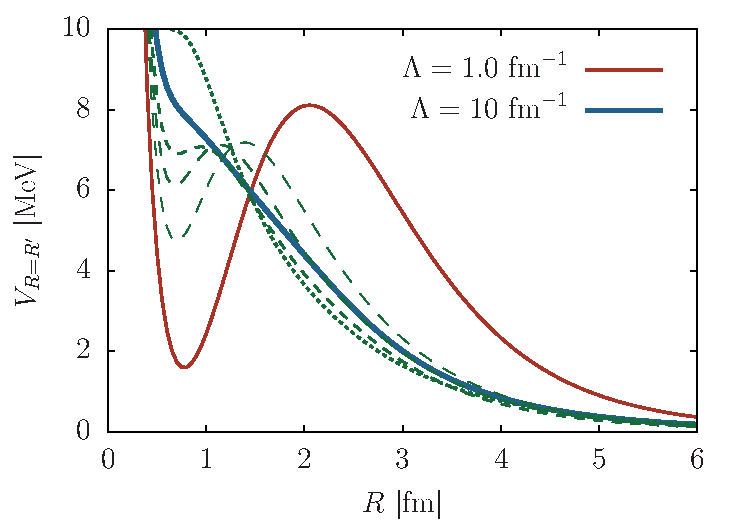
\includegraphics[width=0.95\textwidth]{./Graphs/rgm_potential_nucl} 
\caption{Two-fragment potential as a function of the distance between a
neutron and the center of mass of a triton. The plot shows the $P$-wave component of the
interaction including local and non-local part of the kinetic-, pair-, and three-body interactions.
The non-local parts are evaluated at $R=R'$. The height of the potential's barrier shrinks continuously from
the smallest cutoff (red) and eventually vanishes at the largest (fat blue), with intermediate values represented by green, dashed curves.}
\label{fig:rgm_potential}
\end{figure}
%
%\begin{figure*}[th]
%\captionsetup{width=.4\linewidth,justification=raggedright}
%\begin{tabular}{cc}
%\begin{minipage}[t]{0.45\linewidth}
% 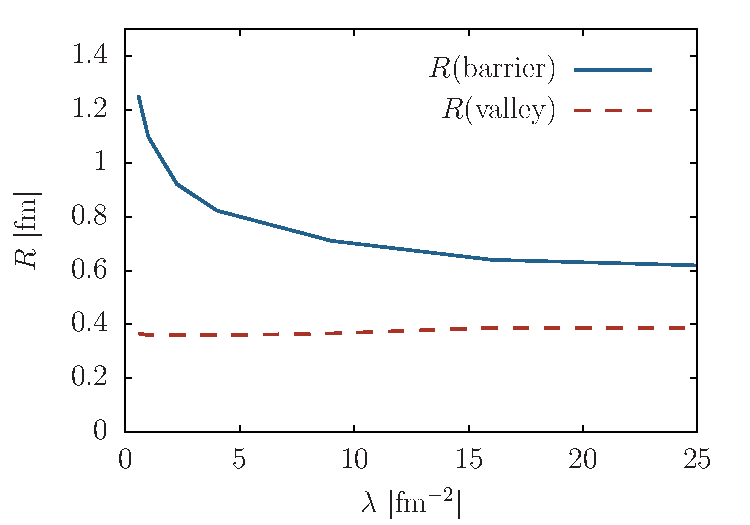
\includegraphics[width=\textwidth]{./Graphs/rgm_potential_MinMax}
% \caption{Locus of the valley (red, dashed) and the barrier (blue, solid) of the effective resonating-group
% interaction (\figref{fig:rgm_potential}) as a function of the regulator parameter $\lambda$.}
%\label{fig:rgm_pot_minmax}
%\end{minipage}
%&
%\begin{minipage}[t]{0.45\linewidth}
% 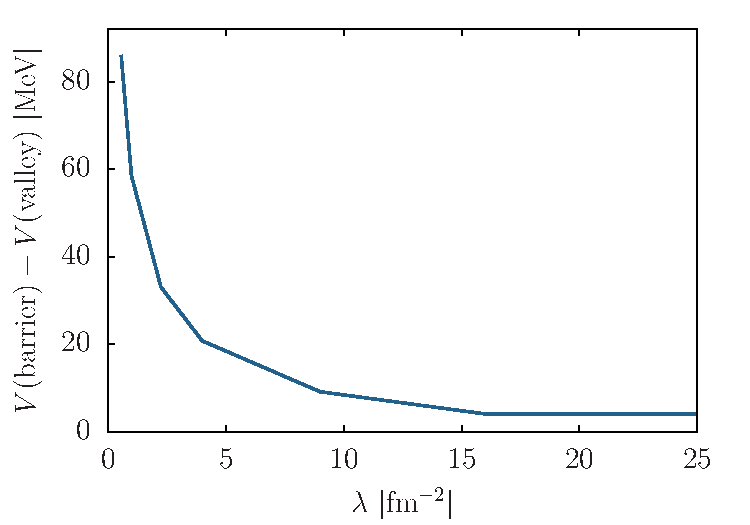
\includegraphics[angle=90,width=\textwidth]{./Graphs/rgm_potential_DeltaMinMax}
%\caption{Regulator dependence of the difference between the first local maximum of the effective resonating-group potential
%(\figref{fig:rgm_potential}) and its first local minimum.}
%\label{fig:rgm_pot_valbardiff}
%\end{minipage}
%\end{tabular}
%\end{figure*}

\end{document}